% !TEX root = dissertation_BB.tex
%% spellcheck-language en-US

%   #
%  ##
%   #
%   #
%  ###

\chapter{Light-sheet imaging of mammalian development}

\graphicspath{{./figures/1_spim/}}

Unraveling the secrets of mammalian development has been a long standing challenge for developmental biologists and medical professionals alike. Understanding early embryonic development allows to shed light on questions such as human infertility and congenital diseases \cite{todo}. 
This phase of early life is an incredibly complex and dynamic process spanning through large scales in space and time. Subcellular processes at the nanoscale are happening in the range of milliseconds or faster, while whole embryo reorganizations and tissue migration events take place over the course of hours \cite{gilbert_developmental_2013}. Resolving these processes presents a true challenge, since to also understand the underlying mechanisms molecular specificity is just as crucial as high spatial and temporal resolution.

Fluorescence microscopy \cite{diaspro_optical_2011}

The most commonly used model organism for these kind of questions is the mouse embryo, that exhibits several common features to human development, and allows to study it 
It has several advantages: full genome is sequenced \cite{mouse_genome_sequencing_consortium_initial_2002}, relatively fast reproduction rate facilitating genetic modifications, already extensively developed tools for genetics and handling \cite{capecchi_new_1989,silver_mouse_1995}. All of these make the mouse embryo the primary model organism when investigating biological processes in mammalians.

fixed samples, histology, immunofluorescence -> no time lapse

ex vivo embryo culture

Hooke's Micrographia 1665 \cite{hooke_micrographia:_1665}

Marvin Misky confocal microscope, no laser, moving smaple \cite{minsky_microscopy_1961}
first laser scanning confocal: sample stationary, objective is moved Davidovits and Egger \cite{davidovits_scanning_1969}
first application of laser scanning confocal in "observation of endothelial cells lining the inside of the cornea" \cite{davidovits_photomicrography_1973}

Imaging mouse embryonic development is an extremely challenging task, due to the intrauterine development of embryos. Although this prevents direct access to the embryos, for some developmental stages it is possible to culture them in an \textit{ex vivo} environment using special media and carefully controlled environmental conditions \cite{garcia_live_2011,doherty_culture_2000}. A second hurdle, aside from \textit{in vitro} culturing, arises from the extreme light sensitivity \cite{nowotschin_chapter_2010} of these embryos, hindering the possibility of long term time-lapse experiments in standard confocal microscopes. Even a few hours of imaging every \SI{15}{mins} can impair or arrest normal development \cite{strnad_inverted_2016}.

Despite these difficulties, numerous studies successfully used confocal microscopy to image live embryos in an \textit{ex vivo} environment, although these studies typically only 

mostly wide-field, Oct4 - self renewal of pluripotent stem cells in ICM/epiblast \cite{nichols_formation_1998}

Sox2 in ICM, also maternal proteins important, similar role as Oct4 Both Oct4 and Sox2 are necessary for ICM formation, without cells become trophoectoderm. Furthermore, for extraembryonic endoderm (ExEn) only Oct4 is required, while for extraembryonic ectoderm (ExE) only Sox2 is required. No time lapse, but confocal used to locate proteins in embryo \cite{avilion_multipotent_2003}

inactivation of X chromosome and histone macroH2A1
mouse liver in confocal - fixed samples \cite{costanzi_histone_1998}

antibodies against amyloid $\upbeta$-peptide reduce Alzheimer in mouse, cryostat sections of mouse brain imaged in confocal\cite{bard_peripherally_2000}


aorta imaging in embryo slices, confocal, live stem cells from aorta endothelium? \cite{boisset_vivo_2010}

fixed embryos, maintaining pluripotency in embryonic stem cells\cite{sato_maintenance_2004}

imaging thrombus formation in real time with intravital high-speed confocal microscopy\cite{falati_real-time_2002}

turning blood into brain hematopoietic stem cells migrate to brain and express neuron-specific antigens \cite{mezey_turning_2000}

papers from Takashi:
apical domain for symmetry breaking \cite{korotkevich_apical_2017}

Asymmetric division of contractile domains couples cell positioning and fate specification, Jean-Léon + Hervé \cite{maitre_asymmetric_2016}

specification of first embryonic lineage, venus trap \cite{dietrich_venus_2015}

surface tension and compaction \cite{maitre_pulsatile_2015}

self organization framework for symmetry breaking (review)


uj regi cikk Keller \cite{keller_life_2006}


Light microscopy is one of the oldest methods that is still widely used today to investigate the inner workings of microscopic life. Light-sheet microscopy is a relatively new addition to the arsenal of tools that comprise light microscopy methods, and is especially suitable for live imaging of embryonic samples over extended periods of time \cite{krzic_multiview_2012,tomer_quantitative_2012}. It is also easily adapted to the sample, allowing to image a large variety of specimens, from entire organs, such as cleared mouse brains \cite{dunsby_optically_2008}, to the subcellular processes occurring inside cultured cells \cite{capoulade_quantitative_2011}.

%\section{Light-sheet microscopy}

\section{Wide-field fluorescence microscopy}
  Fluorescence microscopy \cite{lichtman_fluorescence_2005}, as a subset of light microscopy is one of the few methods that allow subcellular imaging of live specimens. As the name of the technique suggest, this method collects fluorescent light from the specimens which has numerous advantages, but also some drawbacks. Since biological tissue is usually not fluorescent, except for some autofluorescence at shorter wavelengths, fluorescent dyes or proteins have to be introduced to the system in order to be able to collect the necessary information.

  A fluorescent molecule is capable of absorbing photons in a given range (excitation spectrum) and temporarily store its energy by having an electron in  a higher energy orbital, \textit{i.e.} in an excited state. This excited state, however is not stable, and the electron quickly jumps back to the ground state while emitting a photon with equal energy to the energy difference between the excited and ground states. The energy of the absorbed and emitted photons are not the same, however. Energy loss occurs due to internal relaxation events, and the emitted photon has lower energy than the excitation photon. This phenomenon is called the Stokes shift, or red shift \cite{stokes}, and can be exploited in microscopy to drastically increase the signal to noise ratio by filtering out the illumination light (Fig. \ref{fig:spectrum}).

  \begin{figure}
    \centering
    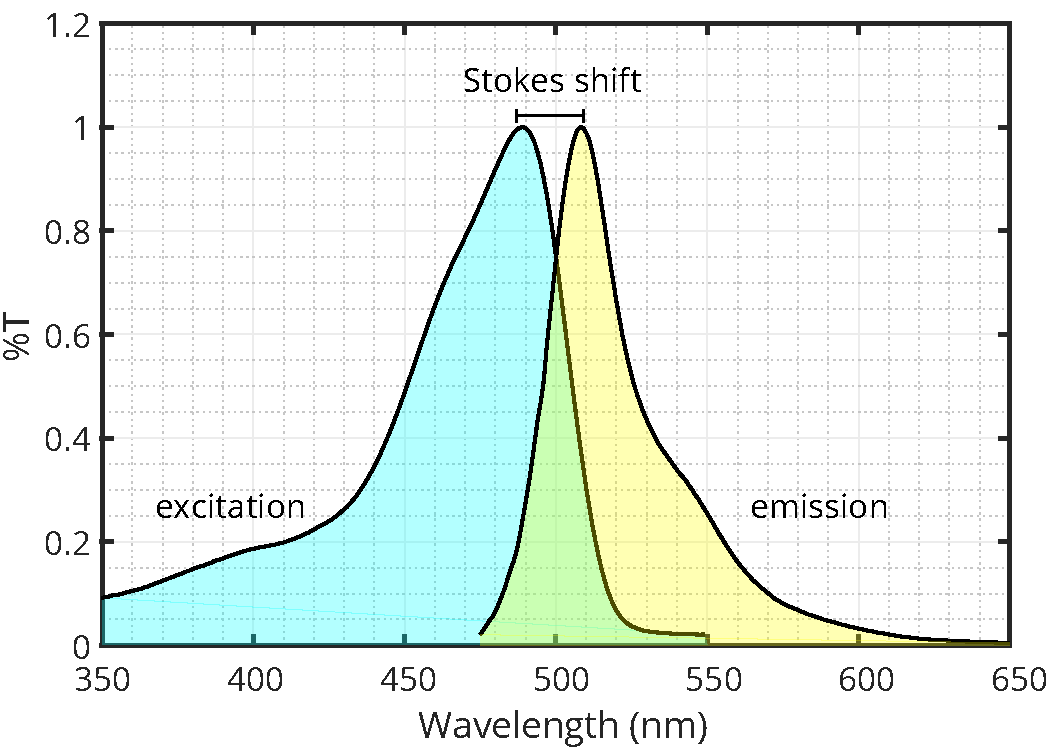
\includegraphics[width=0.6\textwidth]{spectrum/egfp}
    \bcaption[Excitation and emittion spectrum of enchanced green fluorescent protein (EGFP)]{Excitation spectrum in blue, emission spectrum in yellow. The separeation between the two spectra is due to the Stokes shift, which is 19 nm for EGFP. Data from \cite{noauthor_spectra_nodate}. Emitted and excitation light can be separated by a long-pass filter at \SI{500}{nm}.}
    \label{fig:spectrum}
  \end{figure}

  % Although this process can disturb the natural environment 

  %  very small amount of illumination photons will result in fluorescence ($<0.0001\%$), the signal to noise ratio of the fluorescence is still very high due to the filtering.

  \subsection{Fluorescent proteins}
    Traditionally synthetic fluorescent dyes were used to label certain structures in the specimens. Some of these directly bind to their target, such s DAPI to DNA, and others can be used when conjugated to an antibody specific to the structure of interest. The drawback of these methods is that the fluorescent label has to be added to the sample from an external source, and in many cases this also necessitates sample preparation techniques incompatible with live imaging, such as fixation \cite{!!!}.

    The discovery of fluorescent proteins have revolutionized fluorescence microscopy. Since these molecules are proteins, they can be produced directly by the organism if the proper genetic modifications are performed. Even though this was a hurdle at the time of discovering the green fluorescent protein (GFP) \cite{shimomura_extraction_1962}, the first of its kind, genetic engineering techniques evolved since then \cite{prasher_primary_1992}, and not only has it been successfully integrated in the genome of nematodes \cite{chalfie_green_1994}, zebrafish \cite{amsterdam_aequorea_1995}, and mice \cite{okabe_green_1997}, but many variants have been also engineered by introducing mutations to increase fluorescence intensity, and to change the fluorescent spectrum to allow multicolor imaging \cite{heim_wavelength_1994,heim_engineering_1996,cormack_facs-optimized_1996,okabe_green_1997}. The usefulness and impact of these proteins are so profound, that in 2008 the Nobel Prize in chemistry was awarded to Osamu Shimomura, Martin Chalfie, and Roger Tsien ``for the discovery and development of the green fluorescent protein, GFP" \cite{service_three_2008}.
    
    % Discovery and purification of green fluorescent protein from \textit{Aequorea victoria} 
    % cloning of GFP  cDNA 
    % first GFP applications as in vivo cell markers: nematodes , zebrafish , mouse 

    % good for live, naturally fluorescent structures

    % autofluorescence not specific
    % fluorescent dyes
    % fluorescent proteins
    % lot of fluorescent proteins since then \cite{shaner_guide_2005}. 
    % benefits: cell is producing
    % using genetic techniques possible to bind to other proteins, and specifically label structures of interest


  \subsection{Wide-field image formation}
    By imaging fluorescently labeled specimens, a wide-field fluorescence microscope has the capability of discriminating illumination light from fluorescent light due to the Stoles shift described in the previous section. The microscope's operating principle is depicted in Figure \ref{fig:wide-field}.

    A light source, typically a mercury lamp is focused on the back focal plane of the objective to create even illumination at the sample. Before entering the objective, the light is filtered, so only those wavelengths that correspond to the excitation properties of the observed fluorophores are transmitted. Since the same objective is used for both illumination and detection, a dichroic mirror is utilized to decouple the illumination an detection paths. The emitted light is filtered again to make sure any reflected and scattered light from the illumination source is blocked to increase signal to noise ratio.

    Finally, the light is focused by a tube lens to create a magnified image in the camera sensor. This type of imaging is called infinity corrected optics, since the back focal point of the objective is in "infinity", meaning that the light exiting the back aperture is parallel. This is achieved by placing the sample exactly at the focal point of the objective. Infinity corrected optics has the advantage that it allows placing various additional optical elements in the infinity space (\textit{i.e.} the space between the objective and the tube lens) without affecting the image quality. In this example such elements are the dichroic mirror and the emission filter. 

    \begin{figure}[tb]
      \centering
      \includegraphics[page=4,width=0.7\textwidth]{spim_cyl}
      \bcaption[Wide-field fluorescence microscope]{(a) The light source is focused on the back focal plane of the objective to provide an even illumination to the sample. Emitted photons are collected by the objective, and are separated from the illumination light by a dichroic mirror. (b) , $\alpha$}
      \label{fig:wide-field}
    \end{figure}


    The combination of the objective and tube lens together will determine the magnification of the system, it will be the ratio of the focal lengths of these lenses:
    \begin{equation}
      M = \frac{f_{TL}}{f_{OBJ}}.
      \label{eq:magnification}
    \end{equation}
    The final field of view of the microscope will depend on the magnification, and also on the size of the imaging sensor:
    \begin{equation}
      FOV = \frac{A}{M},
      \label{eq:FOV}
    \end{equation}
    where $A$ is the area of the sensor. 

    Apart from magnification, the most important property of the objective is the half-angle of the light acceptance cone, $\alpha$. This not only determines the amount of collected light, but also the achievable resolution of the system (see next section). This angle depends on the size of the lens relative to its focal length. In other words depends on the aperture of the lens, which is why the expression numerical aperture is more commonly used to express this property of the objective:
    \begin{equation}
      NA = n\cdot \sin \alpha.
      \label{eq:NA}
    \end{equation}

    For small $\alpha$ angles, the following approximation holds true: $\sin \alpha \approx \tan \alpha \approx \alpha$. Thus, the numerical aperture can also be expressed as a ratio of the radius of the lens and the focal length:
    \begin{equation}
      NA \approx n \frac{r}{f},\quad \text{when }\alpha \ll 1.
    \end{equation}
    % This expression also shows the relationship of the numerical aperture and the f-number commonly used in photography to characterize a lens' aperture:
    % \begin{equation}
    %     f\# = \frac{f}{d} \approx \frac{2}{n\cdot NA}
    % \end{equation}



  \subsection{Resolution of a wide-field microscope}
    The resolution of an optical systems is defined by the size of the smallest distinguishable feature on the image. Practically this means the minimum distance between two point like objects so that the two objects can still be resolved. This mainly depends on two factors: the NA of the objective, and the pixel size of the imaging sensor.

    Even if the imaging sensor would have infinitely fine resolution, it is not possible to reach arbitrary high resolutions due to the wave nature of light and diffraction effects that occur at the aperture of the objective. This means that depending on the wavelength of the light, any point source will have a finite size on the image that will limit the resolution. The shape of this image is called the \textit{point spread function}, or PSF, as this function describes the behavior of the optical system when imaging a point like source. This property of lenses was already discovered by Abbe in 1873 \cite{abbe_beitrage_1873}, when he constructed his famous formula for resolution:
    \begin{equation}
      \delta = \frac{\lambda}{2 \cdot NA}.
      \label{eq:abbe}
    \end{equation}
    where $d$ is the smallest distance between two distinguishable features.

    This equation can be also derived from the scalar theory of diffraction using a paraxial approximation (Fraunhofer diffraction, \cite{born_principles_2013}) that describes the intensity of the electric field in the focus of a lens \cite{sheppard_imaging_1987}:

    \begin{equation}
      H(u,v) = C_0 \left| \int_0^1 J_0 (vr)e^{-i\frac{1}{2}\cdot ur^2} rdr \right|^2,
      \label{eq:psf}
    \end{equation}
    where $C_0$ is a normalization constant, and $J_0$ is the zero order Bessel function of the first kind. Furthermore, instead of the commonly used Cartesian coordinates $x$, $y$ and $z$, the following optical coordinates are defined:
    \begin{equation}
      v = \frac{2\pi n  r}{\lambda_0} \sin \alpha, \quad
      u=\frac{8\pi n  z}{\lambda_0} \sin^2 \frac{\alpha}{2}
      \label{eq:substitutions}
    \end{equation}
    where $r = \sqrt{x^2 + y^2}$ is the distance from the optical axis, and $\alpha$ is the light collection angle as shown on Fig. \ref{fig:wide-field}. 

    To determine the lateral resolution of the system, let's substitute $u=0$ as the axial optical coordinate, and evaluate Eq. (\ref{eq:psf}) which will give the intensity distribution inn the focal plane:
    \begin{equation}
      H(0,v) = C_0 \left| \int_0^1 J_0(vr)rdr \right|^2 = \left(2\frac{J_1(v)}{v} \right) ^2,
      \label{eq:airy}==
    \end{equation}
    \begin{figure}
      \centering
      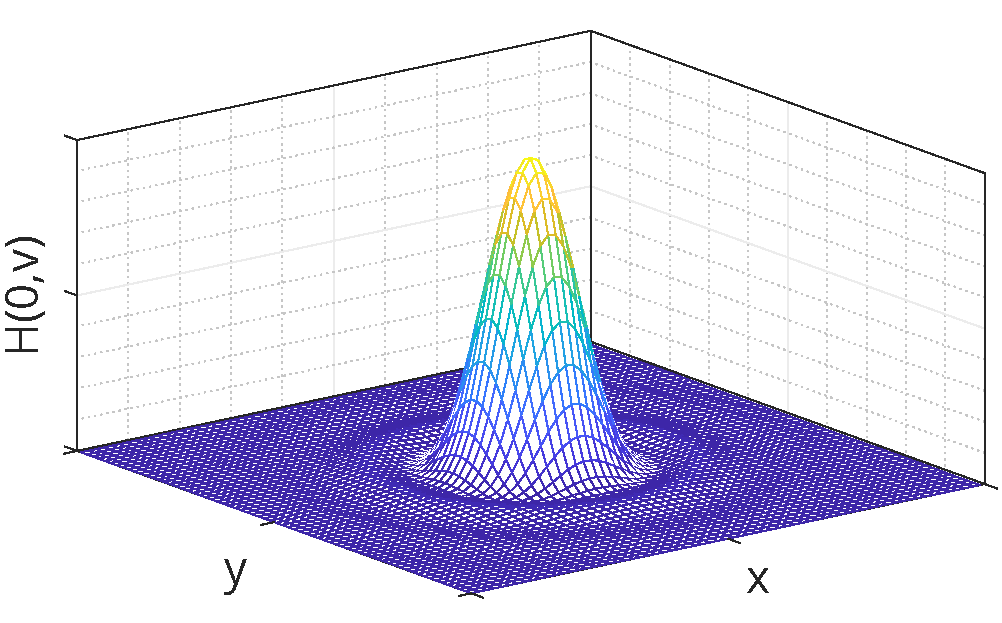
\includegraphics[width=0.7\textwidth]{airy}
      \bcaption[Airy pattern]{Airy pattern calculated in Matlab based on Eq. (\ref{eq:airy})}
      \label{fig:airy}
    \end{figure}


    \begin{figure}
      \centering
      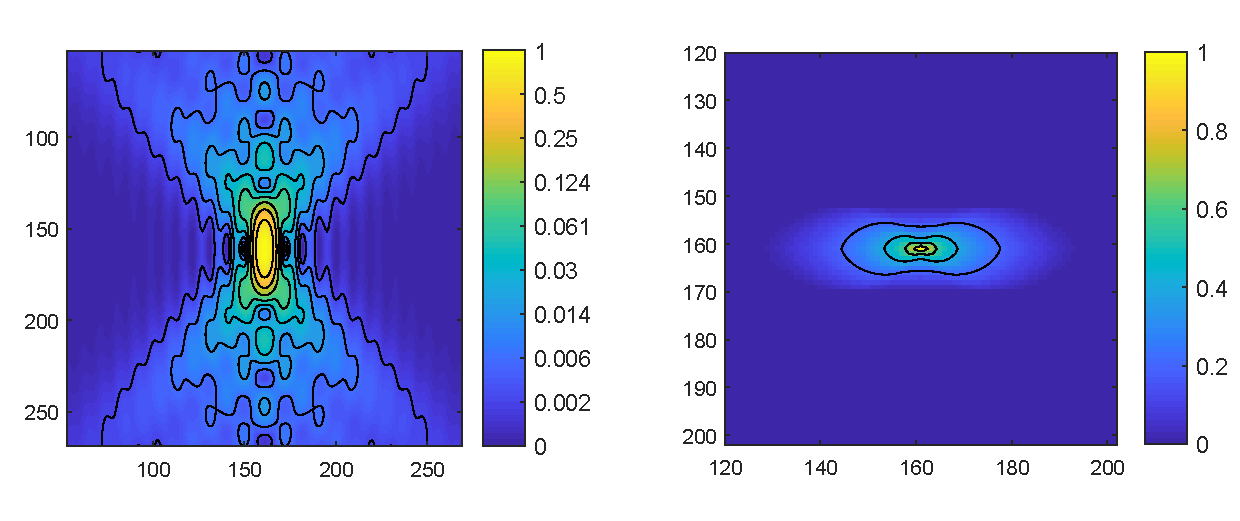
\includegraphics[width=1\textwidth]{psfs/WF.pdf}
      \bcaption[Axial cross section of the PSF and OTF of a wide-field microscope]{Simulated PSF and OTF for a wide-field microscope with a water immersion objective ($n=1.33$). $NA=1.1$, $\lambda = \SI{510}{nm}$}
      \label{fig:psf-wf}
    \end{figure}

    where $J_1$ is the first order Bessel function of the first kind. This equation describes the famous Airy pattern (Fig. \ref{fig:airy}) which will be the shape of the PSF in the focal plane. The width of this pattern is the resolution, and although there are multiple definitions for this, the most commonly accepted is the Rayleigh criterion \cite{rayleigh} which defines the resolution as the distance between the central peak and the first local minimum. As this lies at $v=3.38$, the resolution can be expressed by substituting this value to Eq. (\ref{eq:substitutions}) and calculating the real distance ($r$):
    \begin{equation}
      \delta_{xy} = \frac{3.83}{2\pi} \frac{\lambda_0}{n\cdot \sin \alpha} \approx 0.61 \frac{\lambda_0}{NA},
      \label{eq:lateralRes}
    \end{equation}
    which is equivalent to Abbe's original formula (Eq. (\ref{eq:abbe})). The only difference is the scaling factor which is due to the slightly different interpretations of width of the Airy disk as mentioned earlier.

    Similarly, to calculate the intensity distribution along the axial axis, let's substitute $v=0$ to Eq. (\ref{eq:psf}):
    \begin{equation}
      H(u,0)=C_0\left( \frac{\sin \frac{u}{4}}{\frac{u}{4}}\right) ^2 . 
    \end{equation} 
    For this expression the first minimum lies at $u=4\pi$. Converting back to Cartesian coordinates, the axial resolution can be expressed as:
    \begin{equation}
      \delta_z = \frac{2n\lambda_0}{NA^2}.
      \label{eq:axialRes}
    \end{equation}

    Up till here, we only considered a single, point-like emitter. In a more realistic scenario, however the emitters are neither point-like, nor single. Effectively, however, for every emitter the PSF would be imaged on the sensor, and this creates the final image. In mathematical terms, this can be expressed as a convolution operation between the underlying fluorophore distribution of the object ($O$) and the PSF ($H$):
    \begin{equation}
      I(u,v) = O(u,v) * H(u,v).
    \end{equation}

    The effective result of this kind of diffraction limited image formation is a blurred image with a finite resolution of $\delta_{xy}$ in the lateral direction, and $\delta_z$ in the axial direction.

    The PSF is further affected by the illumination pattern as well. Since the number of emitted fluorescent photons are roughly proportional to the illumination intensity, if the illumination has any structure at the order of the detection resolution, it will have an effect on the overall PSF of the system, which can be expressed as:
    \begin{equation}
      H_{sys} = H_{ill} \cdot H_{det},
      \label{eq:systemPSF}
    \end{equation}
    where $H_{ill}$ is the point spread function of the illumination, and $H_{det}$ is the point spread function of the detection.


\section{Imaging in three dimensions}
  In most cases, a wide-filed microscope is used to image a section of a tissue, thus axial resolution is not a concern. Imaging live specimens, however is not so straightforward, as these samples are usually much thicker than a typical section. For these samples 3-dimensional (3D) imaging is highly beneficial, which necessitates some kind of optical sectioning technique to be able to discriminate the features at different depths.


  Due to the design of the wide-field microscope, any photons emitted from outside the focal plane will also be detected by the sensor, however as these are not originating from the focus, only a blur will be visible. This blur potentially degrades image quality and signal to noise ratio to such extent that makes imaging thick sample very difficult if not impossible in a wide-field microscope \cite{!!!}. 

  % In the previous section we defined optical resolution, and derived the formulas to calculate the lateral and axial resolutions. These formulas, however are not completely accurate for high NA imaging, since the derivation itself depended on a paraxial approximation of the Kirchhoff diffraction equation. A more robust, and generally accepted method to calculate the resolution for high-NA objectives is the Stelzer-Grill-Heisenberg (SGH) theory
  % \cite{grill_method_1999, stelzer_uncertainty_2000}:
  % \begin{equation} \label{eq:latres}
  % \sigma_{xy}=\frac{\lambda}{\sqrt{3-2 \cos \alpha - \cos 2 \alpha}}
  % \end{equation}
  % \begin{equation} \label{eq:axres}
  % \sigma_z = \frac{\lambda}{1-\cos \alpha}
  % \end{equation}

  \begin{figure}
    \centering
    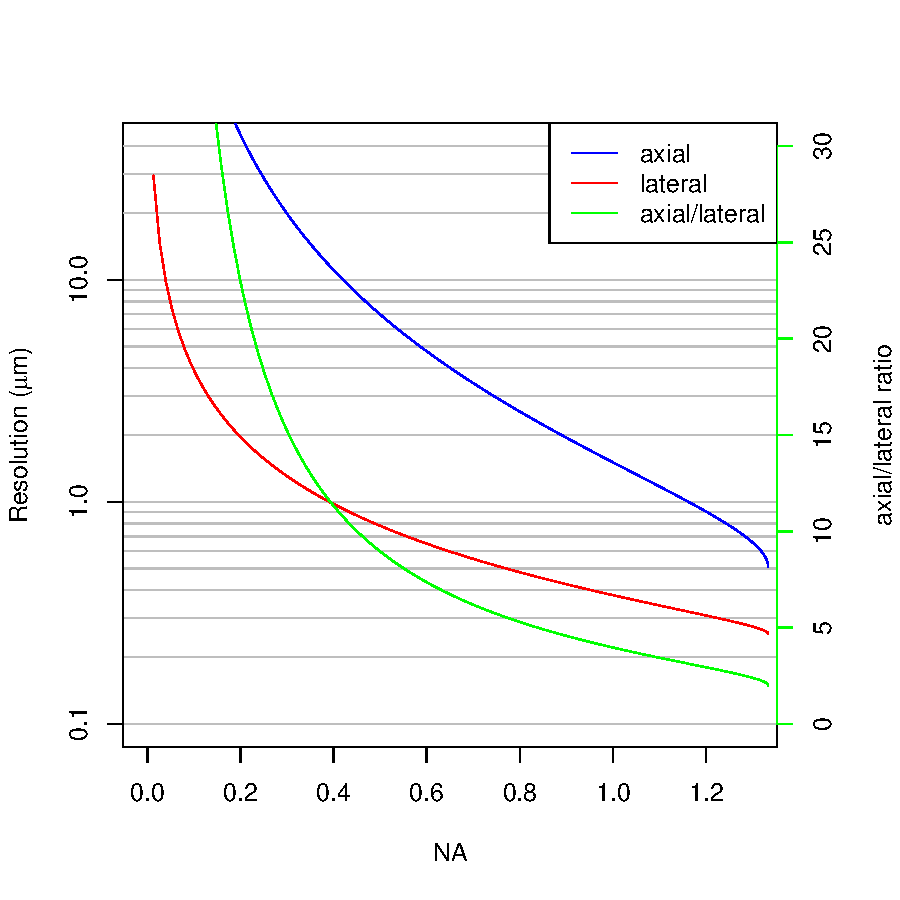
\includegraphics[width=0.6\textwidth]{resolution}
    \bcaption[Resolution of a wide-field microscope]{Axial (blue) and lateral (red) resolutions of a wide-field microscope are shown with respect to the numerical aperture (NA). Resolutions are calculated with $\lambda =510nm$, the emission maximum of GFP and $n=1.33$, the refractive index of water, for water dipping objectives.}
    \label{fig:resolution}
  \end{figure}

  Evaluating Equations (\ref{eq:lateralRes}) and (\ref{eq:axialRes}) for a range of possible numerical apertures reveals the significant differences in lateral and axial resolution for any objective (Fig.~\ref{fig:resolution}). Especially for low NAs, this can be significant, a factor of $\sim$20 difference. For higher (>0.8) NAs the axial resolution increases faster than the lateral, however they will only be equal when $\alpha=\SI{180}{\degree}$. This means that isotropic resolution with a single lens is only possible, is the lens is collecting all light emitting from the sample, which seems hardly possible, and would be highly impractical. For commonly use high NA objectives the lateral to axial ratio will still be around 3--6. 

  Instead of using a single lens to achieve isotropic resolution, it's more practical to image the sample from multiple directions to complement the missing information from different views. When rotating the sample \SI{90}{\degree} for example, the lateral direction of the second view will correspond to the axial direction of the first view. If rotation is not possible, using multiple objectives can also achieve similar result, such as in the case of Multi-Imaging Axis Microscopy (MIAM) \cite{swoger_multiple_2003,swoger_multi-view_2007}. This microscope consisted of 4 identical objectives arranged in a tetrahedral fashion to collect as much light as possible from multiple directions, and provide isotropic 3D resolution, albeit at the expense of extremely difficult sample handling, since the sample was completely surrounded by objectives from all directions. 

  % Another disadvantage of the wide-field microscope, is that it can not be used with thick specimens. Usually this type of microscopy is only used for a single layer of cells, because all the objects in the field of view will appear on the imaging plane, not just the plane in focus. These objects will appear blurred if close to the focus, or just evenly add to the background noise if they are further from the focus. This is why imaging specimens much thicker than $10\ \mu m$ will result in suboptimal image quality.




  \subsection{Laser scanning confocal microscopy}
    Laser scanning confocal microscopy \cite{minsky_microscopy_1961,davidovits_scanning_1969} addresses most of the problems of wide-field microscopy we mentioned in the previous section. It is capable of optical sectioning by rejecting out of focus light, which makes it  true 3D imaging technique. Furthermore, the light rejection also massively reduces out of focus background, and increases contrast.

    This is achieved by two significant modifications compared to the wide-field optical path. To be able to reject the out of focus light, an adjustable pinhole in placed at the focus of the tube lens. Light rays originating from the focal point will meet at this position, and are able to pass through the pinhole, however out of focus light will converge either before or after the aperture, and thus the aperture blocks these rays. To maximize the fluorescence readout efficiency for the single focal point, a photomultiplier tube is used instead of an area sensor (Fig. \ref{fig:confocal}).

    \begin{figure}[tb]
    \begin{subfigure}[t]{0.49\textwidth}
      \centering
      \includegraphics[page=3,width=\textwidth]{spim_cyl}
      \caption{\textbf{Confocal microscope}}
      \label{fig:confocal}
    \end{subfigure}
    \begin{subfigure}[t]{0.49\textwidth}
      \centering
      \includegraphics[page=5,width=\textwidth]{spim_cyl}
      \caption{\textbf{Confocal-theta microscope}}
      \label{fig:conf-theta}
    \end{subfigure}
    \bcaption[Basic optical components of a laser scanning confocal and confocal-theta microscope]{Both type of microscopes use confocal images detection, which means that a pinhole is used to exclude light coming from out of focus points. Light intensity is measured by a photomultiplier for every voxel in the region of interest. The final image is generated on a computer using the positions and recorded intensity values. A regular confocal microscope (\ref{fig:confocal}) uses the same objective for illumination and detection, while a confocal-theta microscope (\ref{fig:conf-theta}) uses a second objective that is rotated by $\vartheta$ around the focus. In this case, $\vartheta = 90^\circ$.}
    \label{fig:confocals}
    \end{figure}

    To maximize the signal from the focal point, the illumination light is also focused here by coupling an expanded laser beam through the back aperture of the objective. This not only increases illumination efficiency (since other, not detected points are not illuminated), but has the added benefit of increasing the resolution as well. This is due to the combined effect of illumination and detection PSF as described in Eq. (\ref{eq:systemPSF}) (Fig. \ref{fig:psf-confocal}). For Gaussian-like PSF-s, the final resolution (along a single direction) can be calculated in the following way:
    \begin{equation}
      \frac{1}{\delta _{sys}^2} = \frac{1}{\delta _{ill}^2} + \frac{1}{\delta _{det}^2},
      \label{eq:systemRes}
    \end{equation}
    where $\delta_{ill}$ and $\delta_{det}$ are the resolutions for the illumination and detection respectively. Since the same objective is used for both illumination and detection, and the difference in wavelength is almost negligible, $\delta_{ill} = \delta_{det} = \delta$, the final system resolution will be:
    \begin{equation}
      \delta_{sys} = \frac{1}{\sqrt{2}} \delta.
    \end{equation}
    This means that the distinguishable features in a confocal microscope are $\sim$0.7 times smaller than in a wide-field microscope using the same objective.

    Because of the different detection method in a confocal microscope, direct image formation on an area sensor is not possible, since at any given time, only a single point is interrogated in the sample. Instead, it's necessary to move the illumination and detection point in synchrony (or in a simpler, albeit slower solution, the to move sample) to scan the entire field of view. The image can be later computationally reconstructed by a computer program that records the fluorescence intensity of every point of the field of view, and displays these values as a raster image.


    \begin{figure}
      \centering
      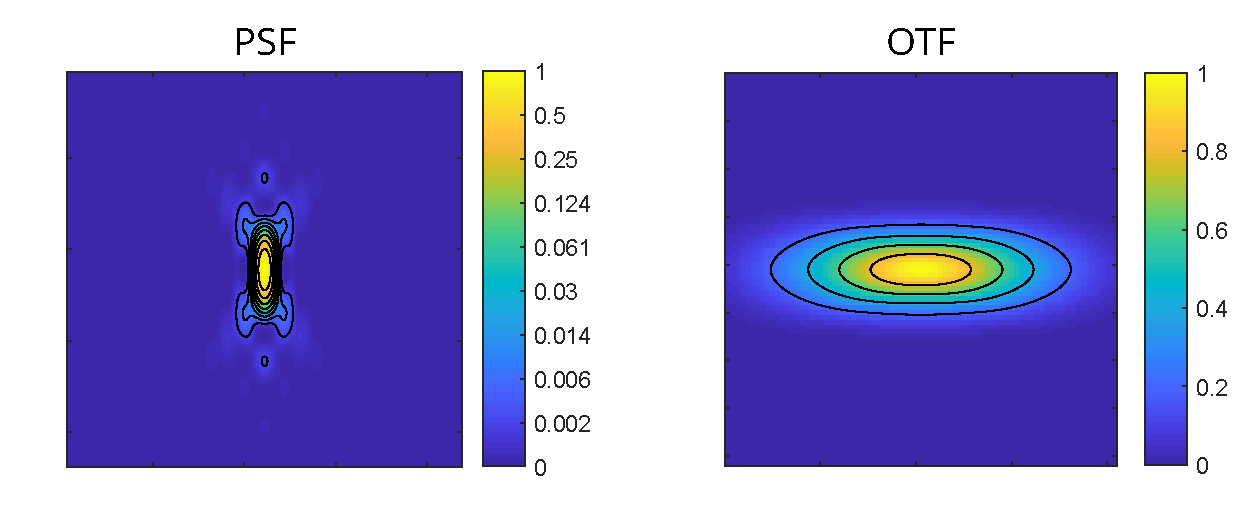
\includegraphics[width=1\textwidth]{psfs/confocal.pdf}
      \bcaption[Axial cross section of the PSF and OTF of a laser scanning confocal microscope]{Simulated PSF and OTF for a laser scanning confocal microscope with a water immersion objective ($n=1.33$). $NA=1.1$, $\lambda = \SI{510}{nm}$}
      \label{fig:psf-confocal}
    \end{figure}


  \subsection{Confocal-theta microscopy}

    % Although confocal microscopy already provides a better resolution in all dimensions, the ratio of the axial and lateral resolution is still very high, due to the single objective illumination and detection. This seriously limits the microscope's 3D imaging capabilities, since in the $z$ direction (i.e. along the imaging axis) the resolution would be significantly worse than in the other directions.
    Although confocal microscopy already has 3D capabilities, it's axial resolution is still limited compared to the lateral, since it uses only one objective. An alternative realization of the confocal microscope, the confocal theta microscope \cite{stelzer_fundamental_1994} introduces a second objective to the system, that is used to illuminate the sample (Figure \ref{fig:conf-theta}). Since this decouples the illumination and detection, using a filter cube is no longer necessary. The second objective is rotated by $\vartheta$ around the focus, this is the where the name of this setup originates from.

    As in the case of standard confocal microscopy, the system PSF is improved by the illumination pattern. Here, however, the axial direction of the detection coincides with the lateral direction of the illumination, which results in a dramatic improvement of axial resolution compared to standard confocal microscopy. Lateral resolution will also be increased, but by a smaller extent, resulting in an almost isotropic PSF, and equal axial and lateral resolution (Fig. \ref{fig:psf-theta}). 

    Although this is a big improvement to confocal microscopy in terms of resolution, this technique did not reach a widespread adoption as it complicates sample handling, while still suffering from two big drawbacks of confocal microscopy techniques that limits its live imaging capabilities.

    Imaging live specimens for an extended period of time with confocal microscopy although possible \cite{aldaz_live_2010, maitre_asymmetric_2016}, is not ideal. For each voxel imaged, a large portion of the specimen has to be illuminated, which results in a very high dose of radiation on the samples. This can be as much as 30--100 times larger, than the dose used for the actual imaging \cite{reynaud_light_2008}. Illumination with high power of laser for an extended time frame can result in bleaching the fluorophores, which in turn will lower the signal at later times. Furthermore, any absorbed photon has the possibility to disrupt the chemical bonds inside the specimen, which can lead to phototoxic effects. Furthermore, the usage of the pinhole although increases resolution, also decreases the detectable signal intensity, thus has a negative impact on image contrast \cite{stelzer_contrast_1998}.




%  ######  ########  #### ##     ## 
% ##    ## ##     ##  ##  ###   ### 
% ##       ##     ##  ##  #### #### 
%  ######  ########   ##  ## ### ## 
%       ## ##         ##  ##     ## 
% ##    ## ##         ##  ##     ## 
%  ######  ##        #### ##     ## 


\section{Light-sheet microscopy}
  \label{sec:light-sheet}
  \begin{figure}[b!]
    \centering
    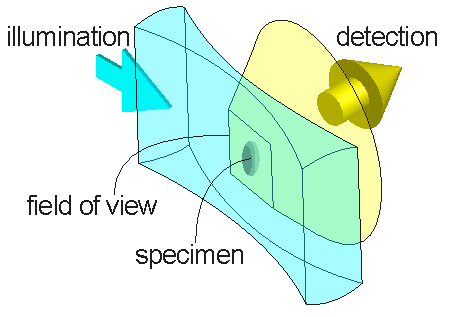
\includegraphics[width=0.6\textwidth]{spim_concept}
    \bcaption[Basic concept of single-plane illumination microscopy]{The sample is illuminated from the side by laser light shaped to a light-sheet (blue). This illuminates the focal plane of the detection lens, that collects light in a wide-field mode (yellow). The image is recorded, and the sample is translated through the light-sheet to acquire an entire 3D stack.}
    \label{fig:spim_concept}
  \end{figure}

  A selective-plane illumination microscope (SPIM) uses a light-sheet to illuminate only a thin section of the sample (Figure~\ref{fig:spim_concept}). This illumination plane is perpendicular to the imaging axis of the detection objective and coincides with the focal plane. This way, only the section in focus will be illuminated, thus providing much better signal to noise ratio. In case of conventional wide-field fluorescent microscopy, where the whole specimen is illuminated, light scattering from different regions contribute to a significant background noise. With selective-plane illumination, this problem is intrinsically solved, and it also provides a true sectioning capability. This makes SPIM especially suitable for 3D imaging.

  

  The main principle behind single plane illumination microscopy, that is illuminating the sample from the side by a very thin light-sheet, dates back to the early 20\textsuperscript{th} century, when Siedentopf and Zsigmondy first described the ultramicroscope \cite{siedentopf_uber_1902}. This microscope used sunlight as an illumination source, that was guided through a precision slit to generate a thin light-sheet. This allowed Zsigmondy to visualize gold nanoparticles floating in and out of the light-sheet. Since these particles are much smaller than the wavelength of the light, the device was called an ultramicroscope. His studies with colloids together with the development of the ultramicroscope led Zsigmondy to win the Nobel Prize in 1925.

  previous to SPIM:
  Voie et al. fixed guinea pig cochlea, rotating and reconstruction in 3D \cite{voie_orthogonal-plane_1993}, called Orthogonal-plane Fluorescent Optical Sectioning. Lateral resolution around \SI{10}{\micro m} and axial resolution of \SI{26}{\micro m}, with very large, \SI{1.5}{mm} field of view. Since the specimens they imaged contained calcium rich bone tissue, optical imaging was only possible by using an optical clearing method. In this work, they used EDTA (ethylenediaminetetraacetic acid) dehydrated in ethyl alcohol, then it was cleared, finally immersed in a fluorescent dye bath. TO acquire 3D images, the specimen was rotated, and translated to compensate for the off-axis rotation.

  follow-up to Voie and Spelman: \cite{voie_three-dimensional_1995} 3D reconstruction of the cochlea for the images

  Similar to SPIM but not fluorescent: light scanning photomicrography \cite{huber_3d_2001}

  Then, in 2002, Fuchs et al. introduces Thin  Light-Sheet Microscopy \cite{fuchs_thin_2002} who use this technique to investigate the microbial life in seawater samples without disturbing their natural environment (by e.g. placing them on a coverslip). Using TSLM allowed the to image the bacteria directly in the staining solution containing SYBR Green I without having to deal with background illumination from the dye, which would have been an issue with confocal microscopy for example. Their light-sheet was similar to the one utilized in OPFOS, being \SI{23}{\micro m} thin, and providing a \SI{1}{mm} \ \SI{1}{mm} field of view.

  The real breakthrough happened when light-sheet microscopy was combined with 
  endogenous fluorescent labels: fluorescent proteins
  live imaging for long time
  and light-sheet
  these techniques were all combined in the 2004 Science paper from Huisken et al. that marks a landmark in light-sheet microscopy, and since then a widespread adoption started  in biological research, with multiple groups implementing their own setups.

  Since then however, light-sheet microscopy was seldom used, but in the last decade it was reinvented and combined with fluorescent microscopy. The first notable light-sheet fluorescent microscope (LSFM) was developed at EMBL in 2004 \cite{huisken_optical_2004}, that demonstrated the benefits of using a light-sheet in imaging developmental processes in three dimension.

  Since then, light-sheet based imaging has gained more and more popularity, as it can be adapted and applied to a wide variety of problems. It was numerously proven to be a better choice than confocal microscopy \cite{reynaud_light_2008,huisken_selective_2009} especially in developmental biological applications \cite{weber_light_2011}. It can also be used with a wide variety of specimens of different sizes, such as zebrafish embryo \cite{keller_reconstruction_2008,kaufmann_multilayer_2012,mickoleit_high-resolution_2014}, mouse brain \cite{dodt_ultramicroscopy:_2007,} or drosophila embryo \cite{krzic_multiview_2012}. It is also possible to use light-sheet microscopy in super-resolution, allowing for individual molecule localization \cite{cella_zanacchi_live-cell_2011}.

  %\begin{itemize}	
  %	\item mSPIM, pivoting light-sheet \cite{huisken_even_2007}
  %	\item omnidirectional microscopy (review) \cite{weber_omnidirectional_2012}
  %	\item SiMView \cite{tomer_quantitative_2012}
  %\end{itemize}

  \subsection{Optics of light-sheet microscopy}

    
    \begin{figure}[htpb]
        \centering
        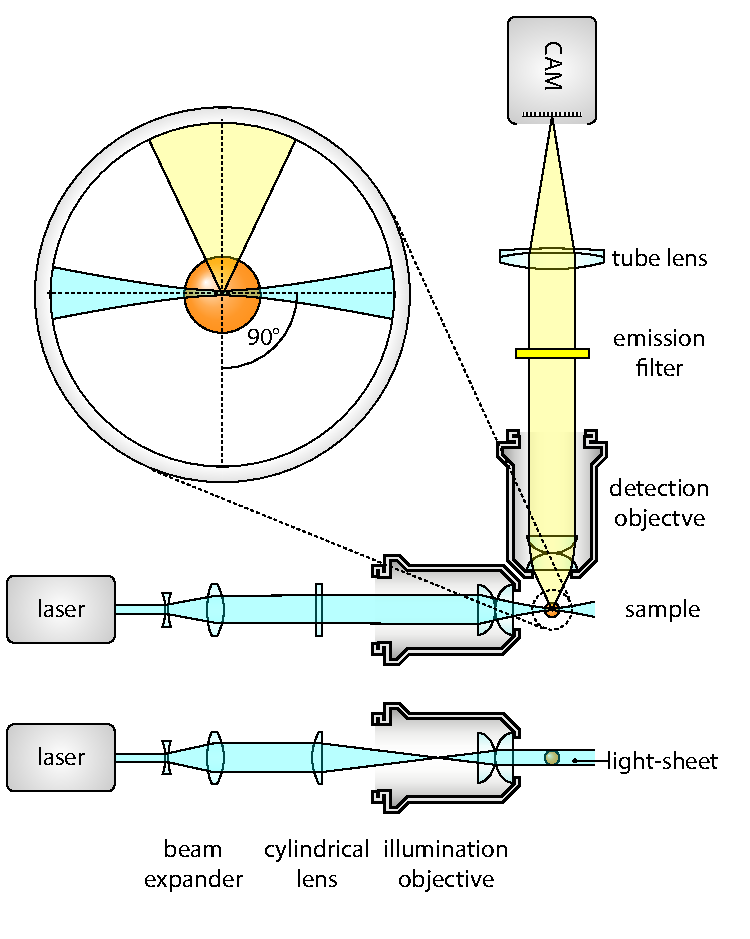
\includegraphics[page=1,width=0.8\textwidth]{spim_cyl}
        \bcaption[Basic optical components of a SPIM]{A selective plane illumination microscope uses two objectives orthogonally aligned. One objective is used to generate a thin light-sheet that illuminates the sample from the side, while the other is used for detection. To generate an image of the specimen, a suitable tube lens is used to focus the light on the sensor of a detection unit (e.g. sCMOS camera). The light-sheet is generated by the illumination objective, using a beam that is previously shaped by a cylindrical lens.}
        \label{fig:light-sheet}
    \end{figure}

    \begin{figure}
        \centering
        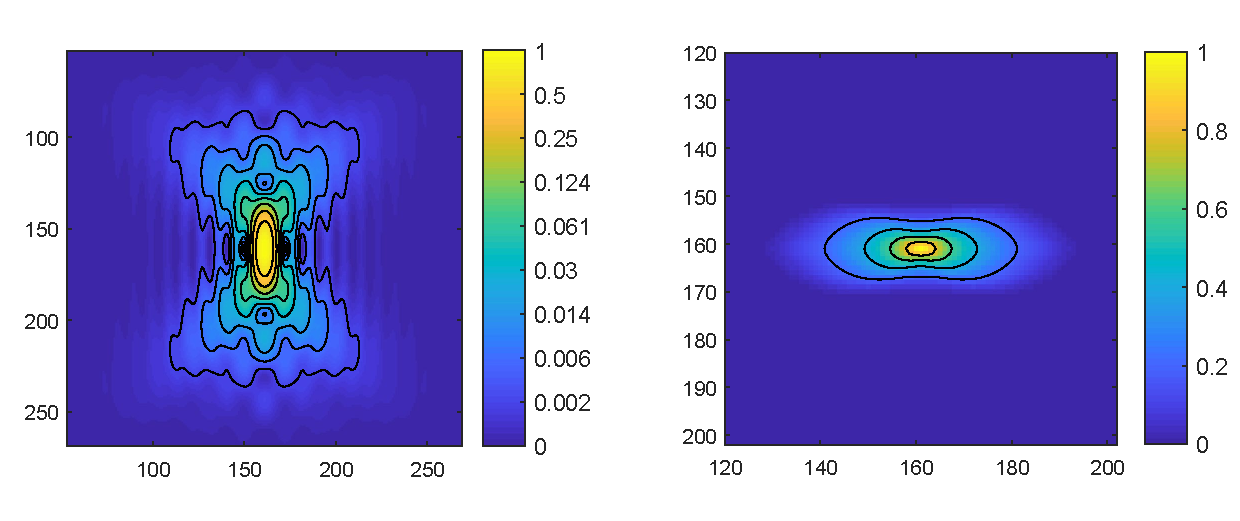
\includegraphics[width=1\textwidth]{psfs/SPIM.pdf}
        \bcaption[Axial cross section of the PSF and OTF of a single plane illumination microscope]{Simulated PSF and OTF for a single plane illumination microscope with a water immersion objectives ($n=1.33$). Detection: $NA=1.1$, $\lambda = \SI{510}{nm}$, Illumination: $NA=0.1$, $\lambda = \SI{488}{nm}$}
        \label{fig:psf-spim}
    \end{figure}


  % \subsection{Detection}
    Since illumination and detection for lght-sheet microscopy are decoupled, two independent optical paths are implemented.

    The detection unit of a SPIM is basically equivalent to a detection unit of a wide-field microscope, without a dichroic mirror (Figure \ref{fig:light-sheet}). Most important components are the objective together with the tube lens, filter wheel, and a sensor, typically a CCD or sCMOS camera.

    One of the most important aspects that determine the resolution of the microscope is the detection objective. Since in developmental biology specimens require a water-based solution, these objectives are usually water dipping objectives directly submerged in the medium. Since the refraction index of water ($n=1.33$) is greater than the refraction index of air, these objectives tend to have a higher $NA$, which results in higher resolution. This, however, also depends on the sensor used, mainly on the pixel size ($d_{sensor}$).

    The magnification is typically $10\times$, $20\times$, $40\times$ or $100\times$ but these values are sound only when the objective is used together with the prescribed tube lens. These lenses are specially made to be used with the specific objectives, and are corrected for any aberrations. They typically have a focal length of 160--200mm.


  % \subsection{Illumination}

    \subsection{Static light-sheet illumination}
      The light-sheet can be generated using a cylindrical lens, which focuses the laser beam in only one direction, and creating a thin sheet in the proximity of the focal point. However, to achieve light-sheets that are thin enough, one would need to use cylindrical lens with low focal lengths, but these are hardly accessible in well corrected formats. For this reason, its more common to use a longer focal length cylindrical lens in conjunction with a microscope objective, which is well corrected for chromatic and spherical aberrations \cite{greger_basic_2007}. This way, the light-sheet length, thickness and width can be adjusted for the specific imaging tasks.

      For paraxial waves, i.e. waves with nearly parallel wave front normals, a general wave equation can be approximated with the paraxial Helmholz equation \cite{krzic_multiple-view_2009, saleh_fundamentals_2007}
      \begin{equation}
        \nabla_T^2 + i 2k \frac{\partial U}{\partial z} = 0
        \label{eq:helmholtz}
      \end{equation}
      where $\nabla_T^2 = \frac{\partial^2}{\partial x^2} + \frac{\partial^2}{\partial y^2}$, $U(\vec{r})$ is the wave-function, $k=\frac{2\pi}{\lambda}$ is the wavenumber and we assume, that the light spreads in $z$ direction.
      
      A simple solution to this differential equation is the Gaussian beam:
      \begin{equation}
        U(r,z) = A_0 \cdot \frac{W_0}{W(z)} \cdot e^{-\frac{r^2}{W^2(z)}}\cdot e^{-i\cdot \phi(r,z)}
      \label{eq:gaussian}
      \end{equation}
      where $A_0$ is the amplitude of the wave, $W_0$ is the radius of the beam waist (the thinnest location on the beam), $r=\sqrt{x^2+y^2}$ is the distance from the center of the beam, $W(z)$ is the radius of the beam $z$ distance from the waist, and $\phi(r,z)$ is the combined phase part of the wave-function. Furthermore:

      \begin{equation}
        W(z) = W_0\sqrt{1+\left( \frac{z}{z_0} \right)^2}
      \end{equation}
      where the parameter $z_0$ is called the Rayleigh-range. This has the following connection with the beam waist:

      \begin{equation}
        z_0 = \frac{\pi W_0}{\lambda}
      \end{equation}
      Which means, the thinner the beam waist, the shorter the Rayleigh-range, that is the beam divergence is faster for more focused beams.

      Intensity of the emitted fluorescence is based on the intensity of the excitation light. In case of a Gaussian beam:
      \begin{equation}
        I(r,z) = U(r,z)\cdot U^*(r,z) = |A_0|^2 \cdot \left( \frac{W_0}{W(z)}\right)^2 \cdot e^{-\frac{2r^2}{W^2(z)}}
      \end{equation}

      Apart from the circular Gaussian beam, the elliptical Gaussian beam is also an eigenfunction of Helmholtz equation (\ref{eq:helmholtz}):
      \begin{equation}
        U(x,y,z) = A_0 \cdot \sqrt{\frac{W_{x,0}}{W_x(z)}} \sqrt{\frac{W_{y,0}}{W_y(z)}} \cdot e^{-\frac{x^2}{W_x^2(z)}} \cdot e^{-\frac{y^2}{W_y^2(z)}} \cdot e^{-i\cdot \phi(x,y,z)}
      \end{equation}

      This beam still has a Gaussian profile along the $x$ and $y$ axes, but the radii are uncoupled, which results in an elliptical beam. Since the beam waist is different along the two axes, the Rayleigh range is also different:
      \begin{align}
        z_{x,0} = \frac{\pi W_{x,0}^2}{\lambda} \\
        z_{y,0} = \frac{\pi W_{y,0}^2}{\lambda}
      \end{align}
      Intensity of the beam is the following:
      \begin{equation}
        I(x,y,z) = U(x,y,z)\cdot U^*(x,y,z) = |A_0|^2 \cdot \frac{W_{x,0}}{W_x(z)} \cdot \frac{W_{y,0}}{W_y(z)} \cdot e^{-\frac{2x^2}{W_x^2(z)}} \cdot e^{-\frac{2y^2}{W_y^2(z)}}
      \end{equation}
      where
      \begin{align}
        W_x(z) = W_{x,0}\sqrt{1+\left( \frac{z}{z_{x,0}} \right)^2}\mathrm{\quad and \quad } W_y(z) = W_{y,0}\sqrt{1+\left( \frac{z}{z_{y,0}} \right)^2}
      \end{align}
      
      \begin{figure}[b!]
        \centering
        \begin{subfigure}[b]{0.7\textwidth}
            \centering
            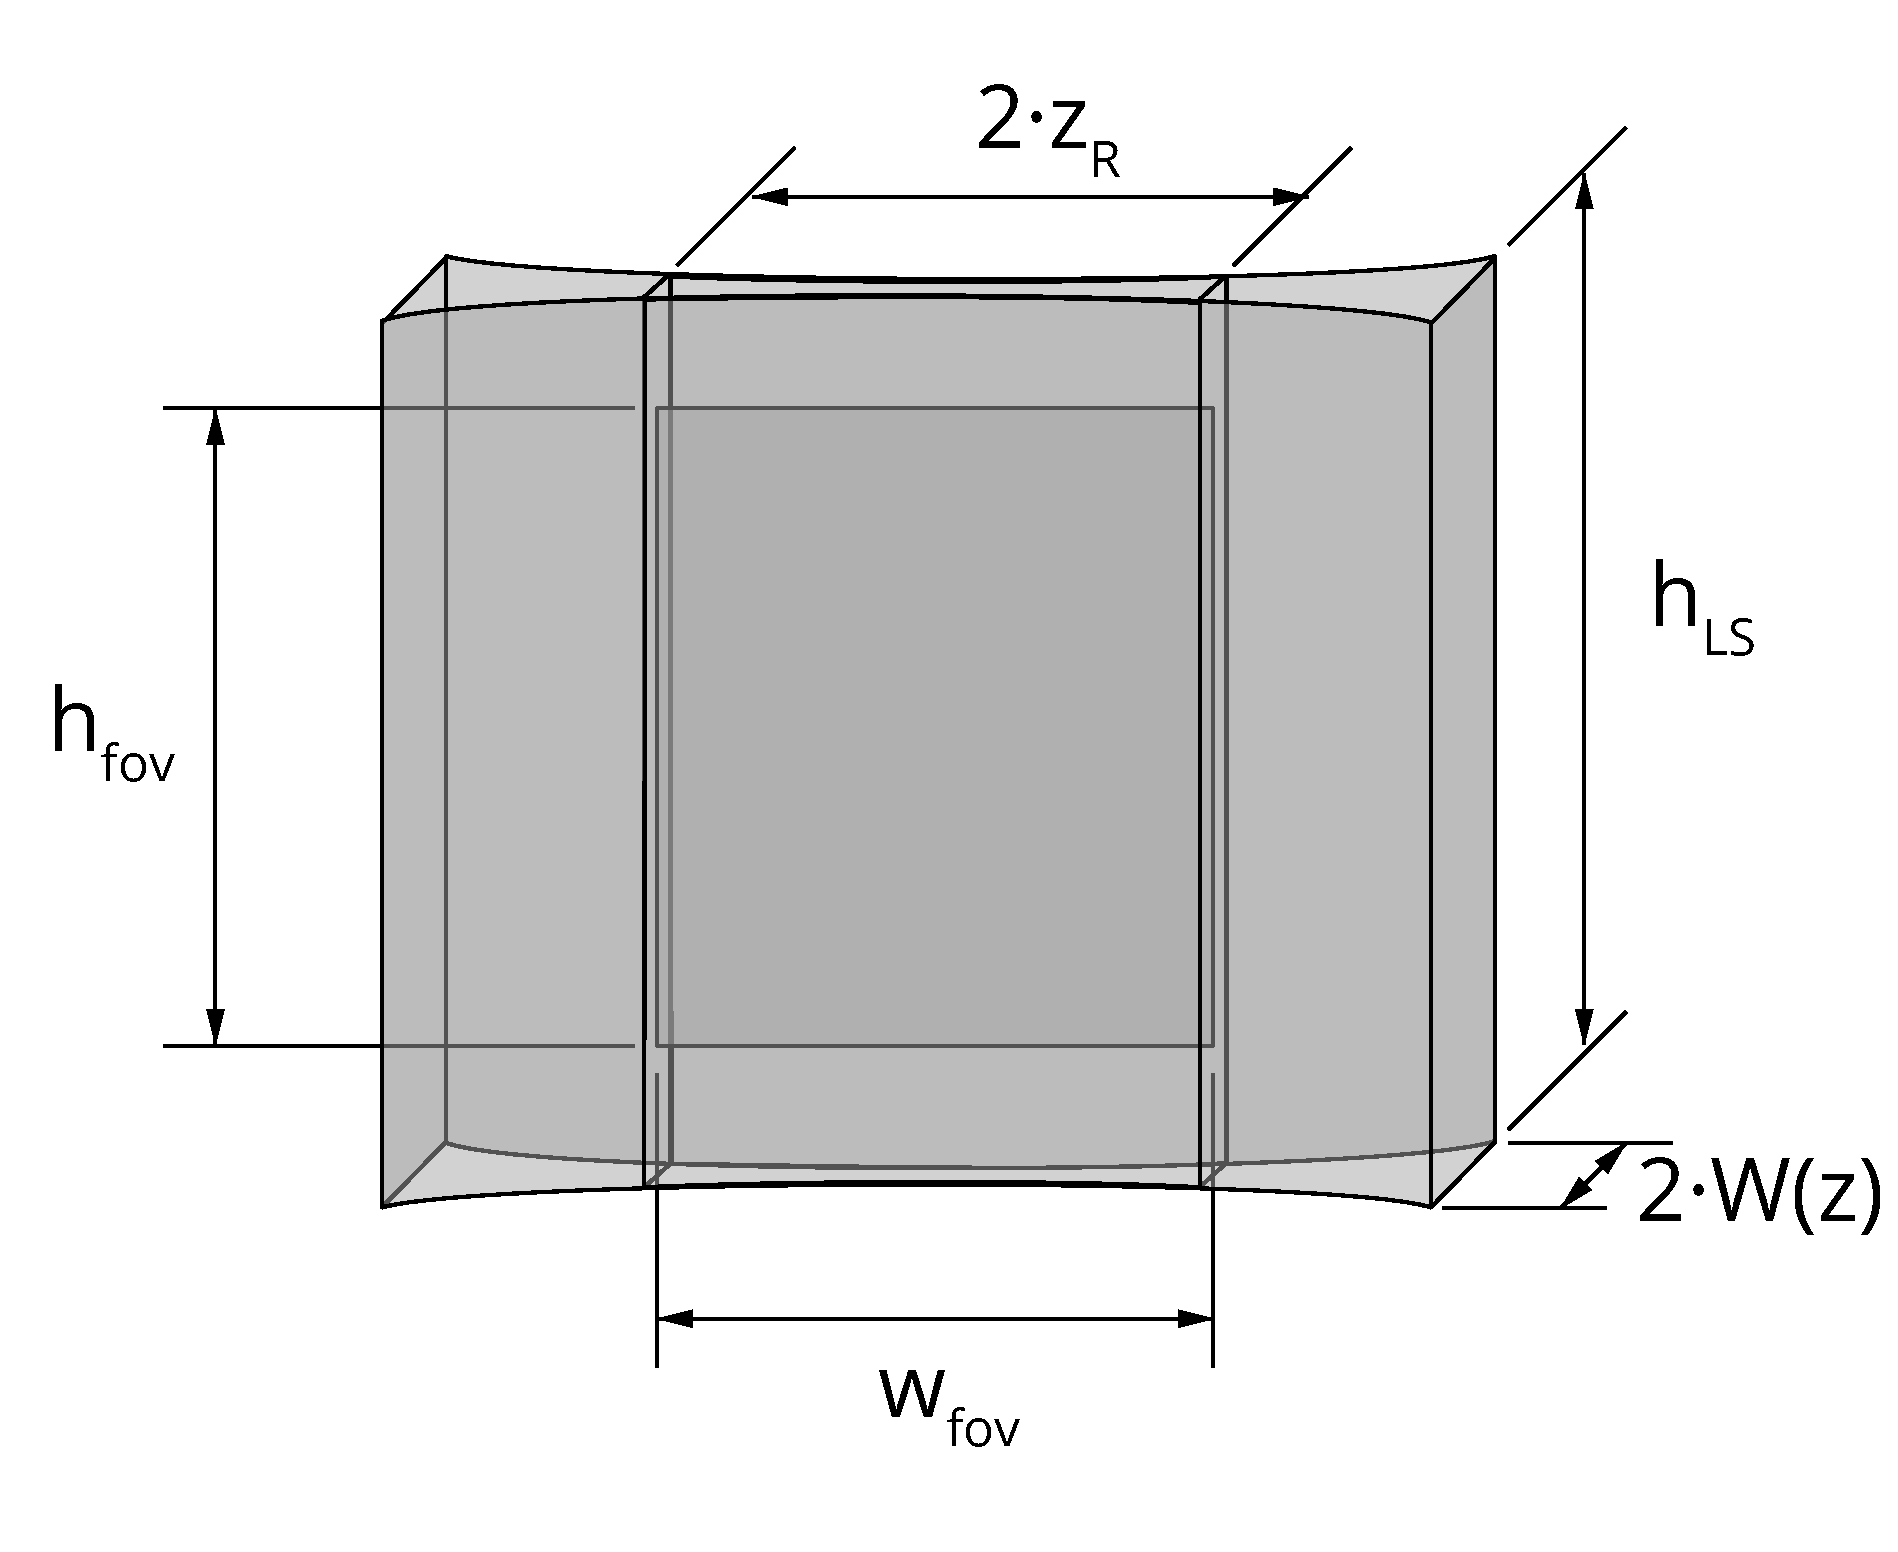
\includegraphics[width=\textwidth]{FOV}
            \caption{}
            \label{fig:fov}
        \end{subfigure}
        \begin{subfigure}[b]{0.49\textwidth}
            \centering
            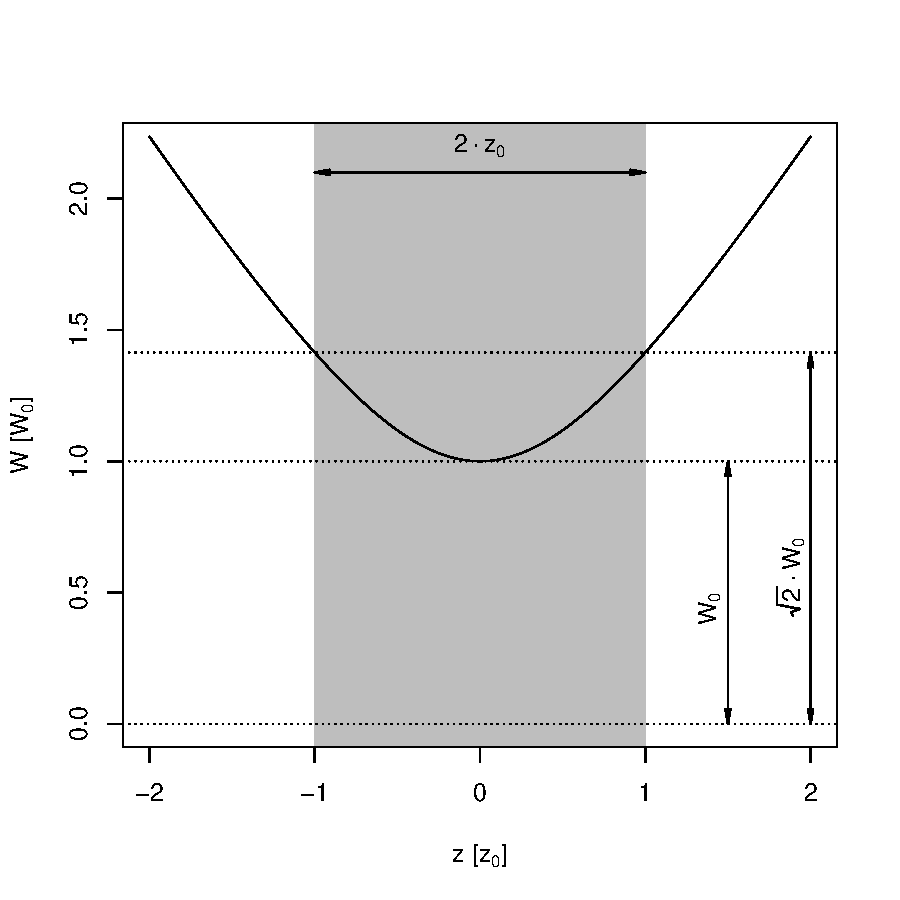
\includegraphics[width=\textwidth]{width}
            \caption{}
            \label{fig:width}
        \end{subfigure}
        \begin{subfigure}[b]{0.49\textwidth}
            \centering
            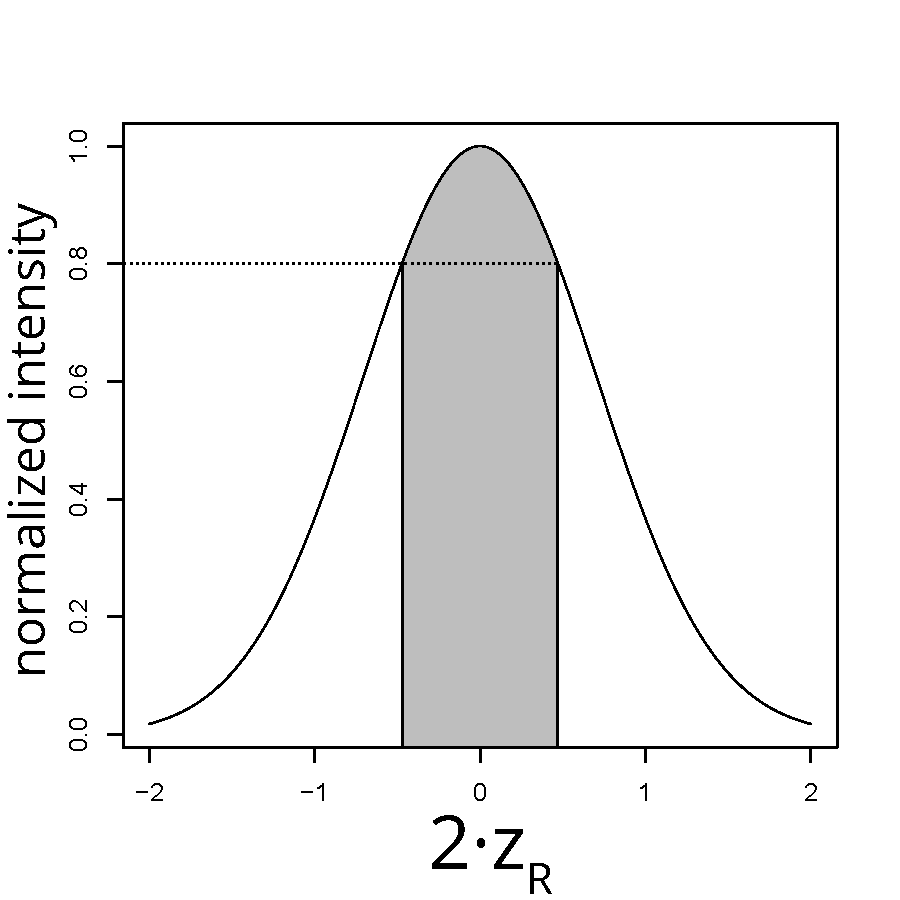
\includegraphics[width=\textwidth]{height}
            \caption{}
            \label{fig:height}
        \end{subfigure}
        \bcaption[Light-sheet dimensions]{ \ref{fig:fov} shows a light sheet, with the field of view indicated. Since the light-sheet intensity is uneven, the field of view has to be confined to a smaller region. \ref{fig:width} The width and thickness of the field of view depends on the Rayleigh length of the beam ($z_{y,0}$). \ref{fig:height} Height of the field of view is determined by the Gaussian profile of the elliptical beam.}
        \label{fig:ls_dim}
      \end{figure}

      Since the illumination is uneven, the usable field of view is smaller than the actual illuminated region (Figure \ref{fig:fov}). The width of the field of view $w_{fov}$ is determined by the Rayleigh length, since this is in a direct relation with the beam divergence. To stay in the optimal region, the light-sheet should only be used in the range of 1 Rayleigh length on both sides of the beam waist (Figure \ref{fig:width}). In this range, the ratio between the thickest (at $z=z_0$) and the thinnest (at $z=0$) part of the beam $W(z)$ will be $\sqrt{2}\approx 1.4142$ which is still acceptable.

      Light-sheet height is determined by the profile of the beam along the vertical axis (Figure \ref{fig:height}). Since this is a Gaussian function (see Equation \ref{eq:gaussian}), only a small part in the middle can be used for imaging, because towards the sides the intensity dramatically drops. To allow a maximum 80\% drop of intensity at the edges, the light-sheet height is $h_{fov}=2\cdot 0.472\cdot W_{x,0}$
      

    \subsection{Digitally scanned light-sheet illumination}
      \begin{figure}[bt!]
        \centering
        \includegraphics[page=2,width=0.8\textwidth]{spim_cyl}
        \bcaption[DSLM illumination]{DSLM illuminates a specimen by a circularly-symmetric beam that is scanned over the field of view. This creates a virtual light-sheet, which illuminates a section of a specimen just like the SPIM. Light-sheet in DSLM is uniform over the whole field of view and its height can be dynamically altered by changing the beam scan range.
      }
          \label{fig:dslm}
      \end{figure}

      Since using cylindrical lenses it's not possible to generate a homogeneous light-sheet, moreover at higher magnification the Rayleigh range would be too small, we also consider using focused beam scanning to generate the light-sheet (digital scanned light-sheet microscopy, DSLM \cite{keller_reconstruction_2008}). To generate a scanning beam, a galvanometer controlled mirror is used to alter the beam path. This can quickly turn around its axis which will result in an angular sweep with the laser beam. To change the angular movement to translation, a scan lens is used to generate an intermediate scanning plane. This plane is then imaged to the specimen by the tube lens and the illumination objective, resulting in a scanned focused beam.

      This method to generate the light-sheet has several advantages compared to a static light-sheet. The height of this sheet is not determined by the cylindrical lens, but it can be dynamically modified. Also, the intensity is uniform through the whole height of the light-sheet.




\section{Multi-view light-sheet microscopy}
  already in 1989 multi-view to increase axial resolution in conventional optical microscope. They imaged \textit{Drosohpila} metaphase plate in Zeiss Axiomat microscope using a 63x 1.2 NA water immersion objective lens. To increase the axial resolution, a special rotation stage was constructed, that allowed rotation around the object of interest to image it from a 90\si{\degree} tilted view. Using a fusion method in the Fourier space, the resolution increased to \SI{0.25}{\micro\meter} in lateral and \SI{0.4}{\micro\meter} in the axial direction for real samples.

  Multiple imaging axis microscopy (MIAM) \cite{swoger_multiple_2003}
  to image specimens from 4 directions in a tetrahedral objective configuration, could reach a 5.8 fold increase in axial resolution by combining the four views as a weighted average.
  Follow up for this: sample manipulation with optical tweezers / optical levitation in 3D \cite{huisken_three-dimensional_2007}(because of the lack of space for mechanical translation stage)
  positioning of a \SI{20}{\micro m} latex bead in a \SI{100}{\micro m} diameter volume by changing the intensity of 4 laser beams. 

  things to improve: resolution
  axial resolution relative to lateral
  complete view
  reduce scattering

  \begin{figure}
    \centering
    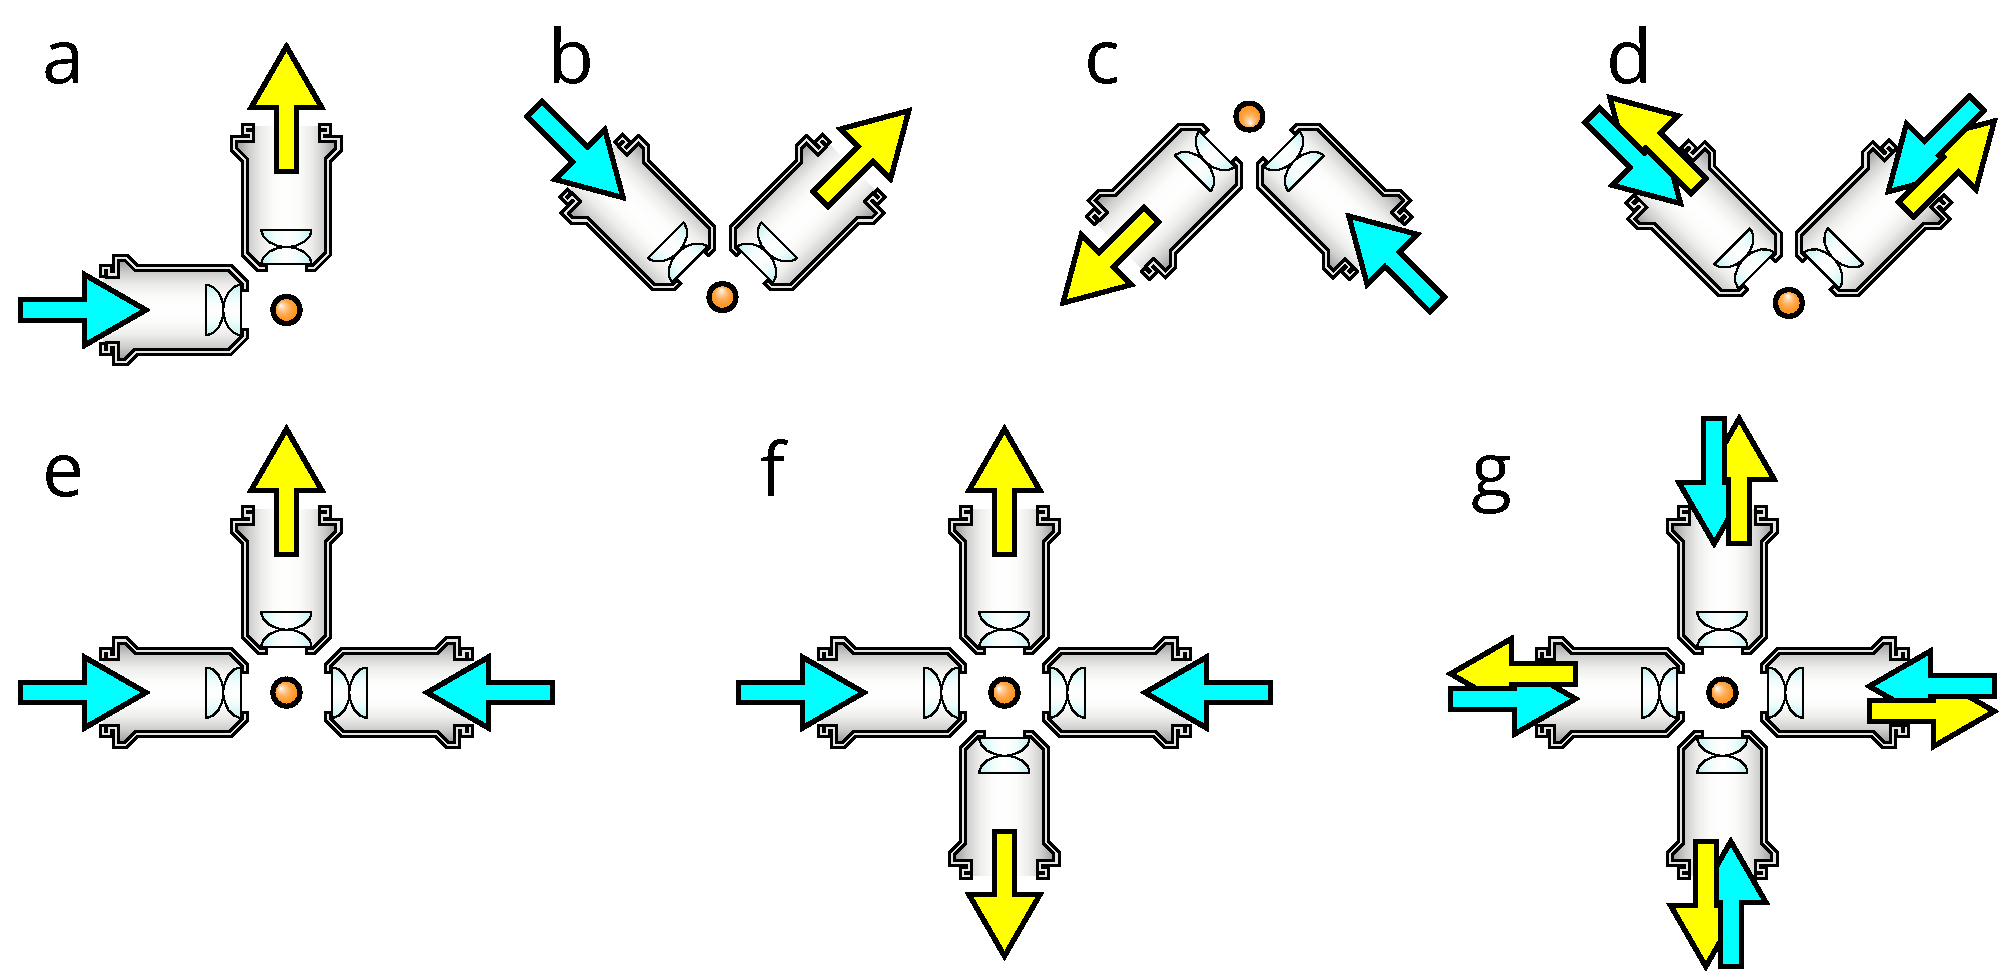
\includegraphics[width=\textwidth]{spim_zoo}
    \bcaption[Different optical arrangements for light-sheet microscopy]{\textbf{(a)} Original SPIM design with a single lens for detection and illuminaiton. \cite{huisken_optical_2004} \textbf{(b)} Upright SPIM to allow for easier sample mounting such as using a petri dish (iSPIM, \cite{wu_inverted_2011, hoyer_breaking_2016}). \textbf{(c)} Inverted SPIM, where the objectives are below the sample, which is held by a thin foil \cite{strnad_inverted_2016}. \textbf{(d)} Dual-view version of the upright configuration, where both objective can be used for illumination and detection (diSPIM, \cite{kumar_dual-view_2014}). \textbf{(e)} Multidirectional-SPIM (mSPIM) for even illumination of the sample with two objectives for illumination \cite{huisken_even_2007}. \textbf{(f)} Multi-view SPIM with two illumination and detection objectives for \textit{in toto} imaging of whole embryos (MuVI-SPIM \cite{krzic_multiview_2012}, SimView \cite{tomer_quantitative_2012}, Four-lens SPIM \cite{schmid_high-speed_2013}). \textbf{(g)} A combination of (d) and (f), using 4 identical objectives, where both can illuminate and detect in a sequential manner, to achieve isotropic resolution without sample rotation (IsoView \cite{chhetri_whole-animal_2015}).}
    \label{fig:spim_zoo}
  \end{figure}